\documentclass[a4paper,11pt]{article}
\usepackage{graphicx}
\usepackage[margin=.5in]{geometry}
\begin{document}

\listoffigures


\begin{figure}[h]
\centerline{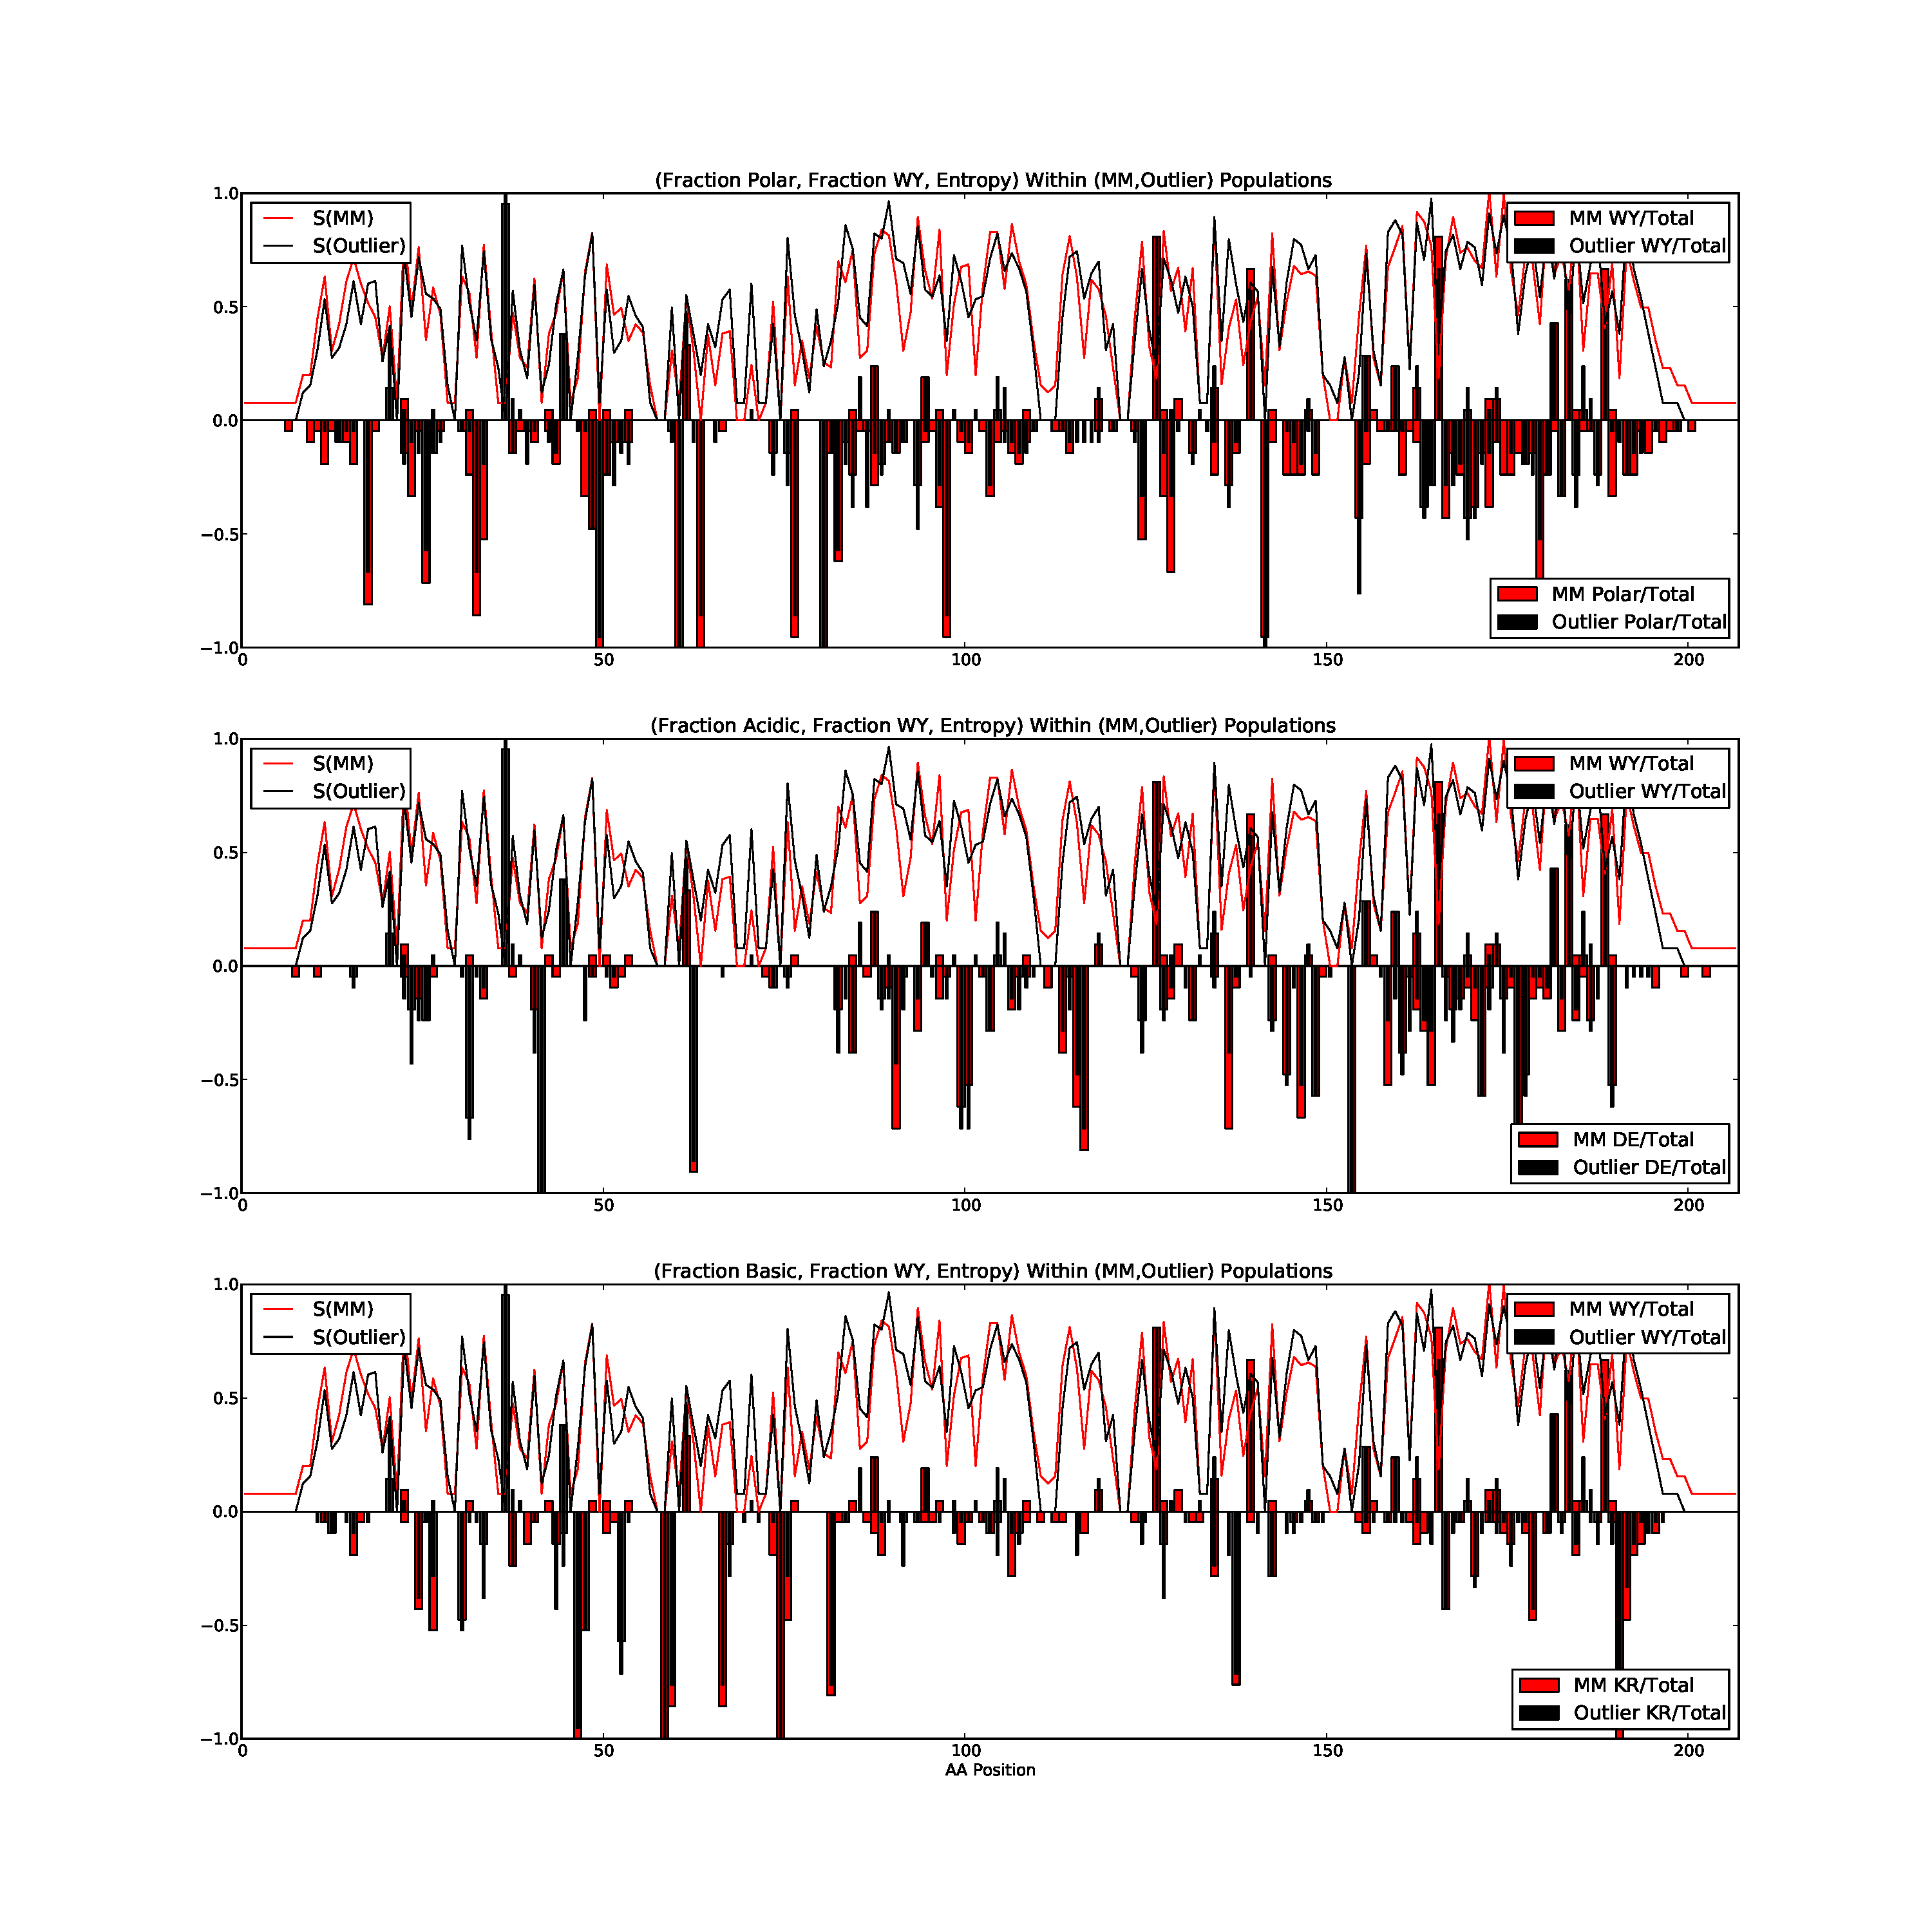
\includegraphics[width=8in]{AA+S.pdf}}
\caption[$S_{\rm red}$, $S_{\rm black}$, WY/Polar/Acidic/Basic Content vs Residue \#]{Entropy and fractional WY/Polar/Acidic/Basic content plotted as a function of position within the DHFR global alignment. Each variable (S, fractional WY content, etc) was plotted simultaneously for both the red grop (DHFR sequences which, upon introduction into E. Coli, conferred Michaelis-Menton obeying behavior) and the black group (DHFR sequences which did not). The entropy of each residue across different DHFR sequences was plotted as a line in the ordinal range [0,1.0] with 1.0 corresponding to 3 bits of entropy. In the same ordinal range of [0,1.0], bars were drawn indicating the fraction of DHFR sequences in the respective red/black groups which contained W or Y residues at that location. Below the horizontal axis, a similar fractional content chart was created indicating the portion of red/black DHFR sequences containing polar, acidic, or basic residues at that location.}
\end{figure}



\begin{figure}[h]
\centerline{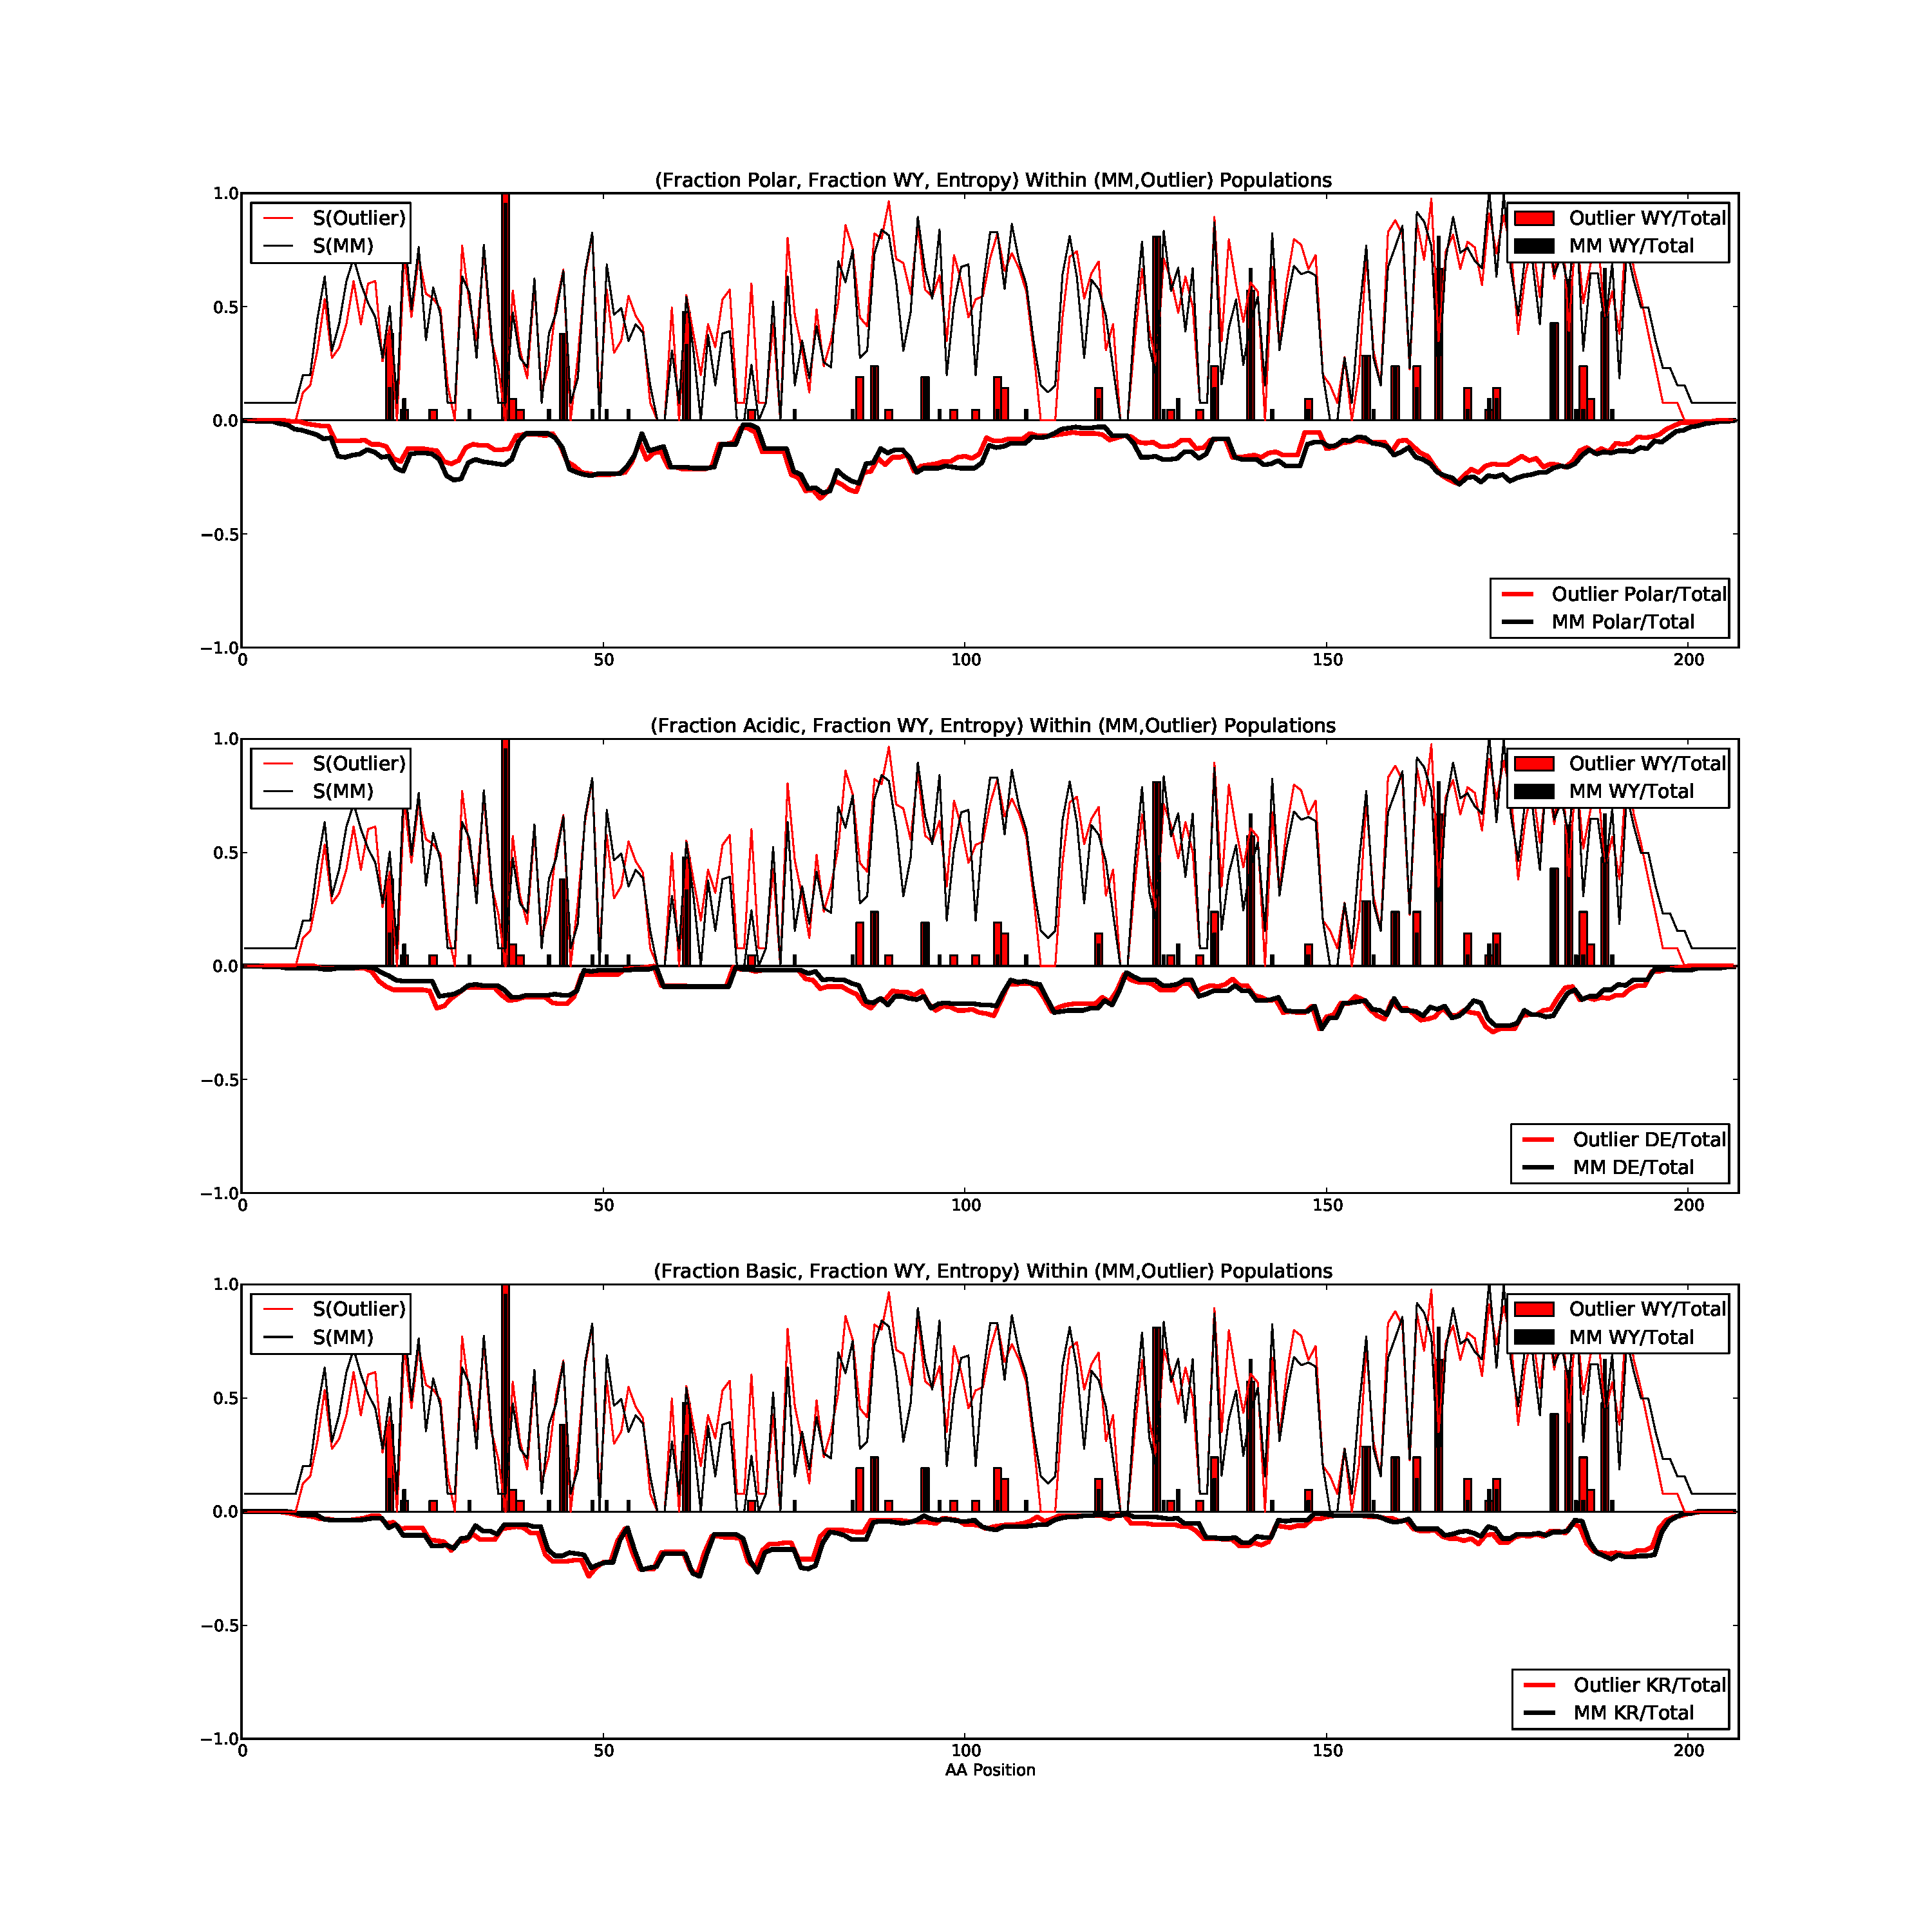
\includegraphics[width=8in]{AA+S_smooth.pdf}}
\caption[$S_{\rm red}$, $S_{\rm black}$, Moving-Average $S_{\rm red}$, Moving-Average $S_{\rm black}$, WY Content vs Residue \#]{Entropy and fractional WY/Polar/Acidic/Basic content plotted as a function of position within the DHFR global alignment. Each variable (S, fractional WY content, etc) was plotted simultaneously for both the red grop (DHFR sequences which, upon introduction into E. Coli, conferred Michaelis-Menton obeying behavior) and the black group (DHFR sequences which did not). The average entropy of each residue across DHFR sequences inside a 20 residue moving window was plotted as a line in the negative ordinal range [-1,0] with -1.0 corresponding to 3 bits of entropy and 0 to 0 bits of entropy. Red/black residue entropy was plotted without a moving average in the positive ordinal range [0,1]. In the same ordinal range of [0,1.0], bars were drawn indicating the fraction of DHFR sequences in the respective red/black groups which contained W or Y residues at that location.}
\end{figure}




\begin{figure}[a]
\centerline{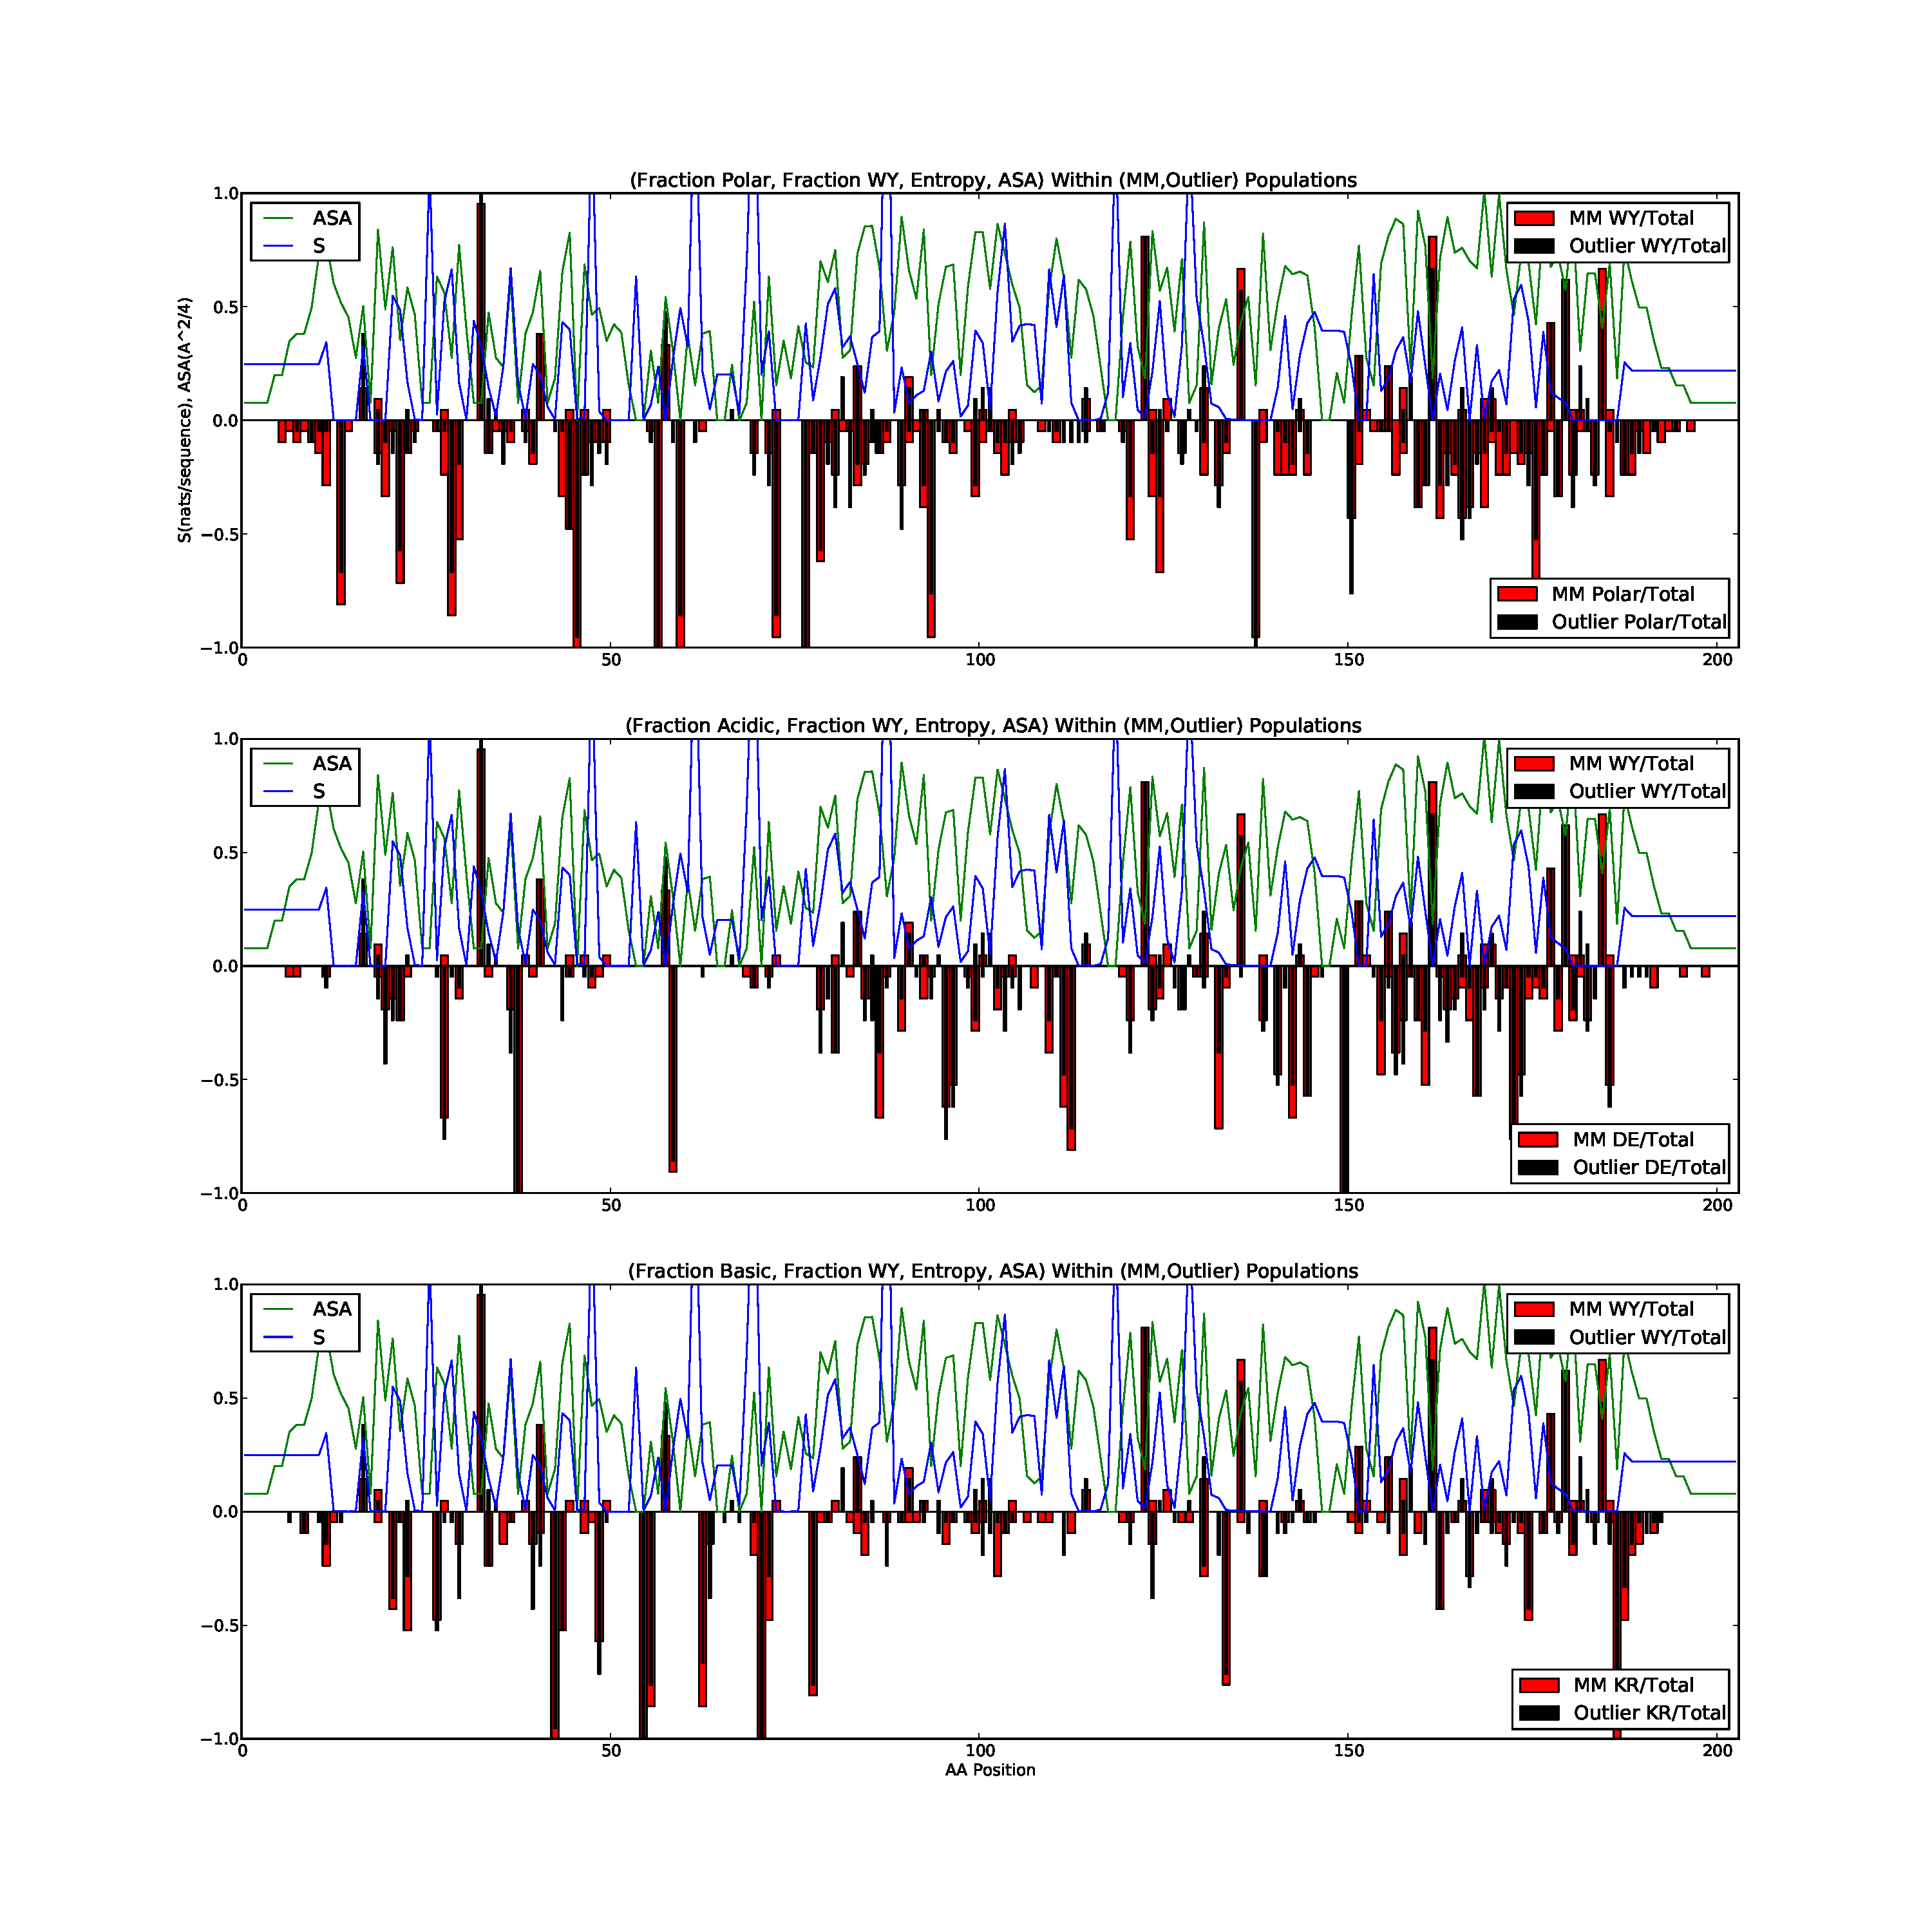
\includegraphics[width=8in]{AA+S+ASA.pdf}}
\caption[$S_{\rm all}$, $ASA_{\rm all}$, WY/Polar/Acidic/Basic Content vs Residue \#]{Accessible Surface Area and Entropy were averaged and plotted as a function of residue \#. For clarity, these averages were taken over all DHFR sequences, rather than over those belonging to the red (Michaelis-Menton obeying) and black (outlier) groups individually, since the averages over red and black groups have extremely high correlation, as can be seen in Figure 1 and Figure 4. A 1.0 ordinal value corresponds to an entropy of three bits. The fractional content of W,Y residues at each position within the red and black groups was plotted using red and black bars in the ordinal range $[0,1.0]$ while an additional class of residue (polar, acidic, or basic) was plotted in the same format in the ordinal range $[-1.0,0]$ using downward-facing bars.}
\end{figure}



\begin{figure}[a]
\centerline{\includegraphics[width=8in]{AA+S+ASA_smooth.pdf}}
\caption[Moving-Average $S_{\rm all}$, Moving-Average $ASA_{\rm all}$, WY/Polar/Acidic/Basic Content vs Residue \#]{Accessible Surface Area and Entropy were averaged over all DHFR sequences and over time (using a 20 residue sliding window), then plotted as a function of residue \#. For clarity, these averages were taken over all DHFR sequences, rather than over those belonging to the red (Michaelis-Menton obeying) and black (outlier) groups individually, since the averages over red and black groups have extremely high correlation, as can be seen in Figure 1 and Figure 4. A 1.0 ordinal value corresponds to an entropy of three bits. The fractional content of W,Y residues at each position within the red and black groups was plotted using red and black bars in the ordinal range $[0,1.0]$ while an additional class of residue (polar, acidic, or basic) was plotted in the same format in the ordinal range $[-1.0,0]$ using downward-facing bars.}
\end{figure}



\end{document}